\documentclass[a4paper,11pt,oneside]{memoir}

% Castellano
\usepackage[spanish,es-tabla]{babel}
\selectlanguage{spanish}
\usepackage[utf8]{inputenc}
\usepackage{placeins}

\RequirePackage{booktabs}
\RequirePackage[table]{xcolor}
\RequirePackage{xtab}
\RequirePackage{multirow}

\usepackage{caption}
\usepackage{subcaption}

% Links
%\usepackage[hidelinks]{hyperref}
% Links
\PassOptionsToPackage{hyphens}{url}%
\usepackage[colorlinks]{hyperref}
\hypersetup{
	allcolors = {blue}
}	

% Ecuaciones
\usepackage{amsmath}

% Rutas de fichero / paquete
\newcommand{\ruta}[1]{{\sffamily #1}}

% Párrafos
\nonzeroparskip

% Enumeraciones multicolumnas
\usepackage{multicol}

% Imagenes
\usepackage{graphicx}
\newcommand{\imagen}[2]{
	\begin{figure}[!h]
		\centering
		\includegraphics[width=0.9\textwidth]{#1}
		\caption{#2}\label{fig:#1}
	\end{figure}
	\FloatBarrier
}

\newcommand{\imagenflotante}[2]{
	\begin{figure}%[!h]
		\centering
		\includegraphics[width=0.9\textwidth]{#1}
		\caption{#2}\label{fig:#1}
	\end{figure}
}



% El comando \figura nos permite insertar figuras comodamente, y utilizando
% siempre el mismo formato. Los parametros son:
% 1 -> Porcentaje del ancho de página que ocupará la figura (de 0 a 1)
% 2 --> Fichero de la imagen
% 3 --> Texto a pie de imagen
% 4 --> Etiqueta (label) para referencias
% 5 --> Opciones que queramos pasarle al \includegraphics
% 6 --> Opciones de posicionamiento a pasarle a \begin{figure}
\newcommand{\figuraConPosicion}[6]{%
  \setlength{\anchoFloat}{#1\textwidth}%
  \addtolength{\anchoFloat}{-4\fboxsep}%
  \setlength{\anchoFigura}{\anchoFloat}%
  \begin{figure}[#6]
    \begin{center}%
      \Ovalbox{%
        \begin{minipage}{\anchoFloat}%
          \begin{center}%
            \includegraphics[width=\anchoFigura,#5]{#2}%
            \caption{#3}%
            \label{#4}%
          \end{center}%
        \end{minipage}
      }%
    \end{center}%
  \end{figure}%
}

%
% Comando para incluir imágenes en formato apaisado (sin marco).
\newcommand{\figuraApaisadaSinMarco}[5]{%
  \begin{figure}%
    \begin{center}%
    \includegraphics[angle=90,height=#1\textheight,#5]{#2}%
    \caption{#3}%
    \label{#4}%
    \end{center}%
  \end{figure}%
}
% Para las tablas
\newcommand{\otoprule}{\midrule [\heavyrulewidth]}
%
% Nuevo comando para tablas pequeñas (menos de una página).
\newcommand{\tablaSmall}[5]{%
 \begin{table}
  \begin{center}
   \rowcolors {2}{gray!35}{}
   \begin{tabular}{#2}
    \toprule
    #4
    \otoprule
    #5
    \bottomrule
   \end{tabular}
   \caption{#1}
   \label{tabla:#3}
  \end{center}
 \end{table}
}

%
% Nuevo comando para tablas pequeñas (menos de una página).
\newcommand{\tablaSmallSinColores}[5]{%
 \begin{table}[H]
  \begin{center}
   \begin{tabular}{#2}
    \toprule
    #4
    \otoprule
    #5
    \bottomrule
   \end{tabular}
   \caption{#1}
   \label{tabla:#3}
  \end{center}
 \end{table}
}

\newcommand{\tablaApaisadaSmall}[5]{%
\begin{landscape}
  \begin{table}
   \begin{center}
    \rowcolors {2}{gray!35}{}
    \begin{tabular}{#2}
     \toprule
     #4
     \otoprule
     #5
     \bottomrule
    \end{tabular}
    \caption{#1}
    \label{tabla:#3}
   \end{center}
  \end{table}
\end{landscape}
}

%
% Nuevo comando para tablas grandes con cabecera y filas alternas coloreadas en gris.
\newcommand{\tabla}[6]{%
  \begin{center}
    \tablefirsthead{
      \toprule
      #5
      \otoprule
    }
    \tablehead{
      \multicolumn{#3}{l}{\small\sl continúa desde la página anterior}\\
      \toprule
      #5
      \otoprule
    }
    \tabletail{
      \hline
      \multicolumn{#3}{r}{\small\sl continúa en la página siguiente}\\
    }
    \tablelasttail{
      \hline
    }
    \bottomcaption{#1}
    \rowcolors {2}{gray!35}{}
    \begin{xtabular}{#2}
      #6
      \bottomrule
    \end{xtabular}
    \label{tabla:#4}
  \end{center}
}

%
% Nuevo comando para tablas grandes con cabecera.
\newcommand{\tablaSinColores}[6]{%
  \begin{center}
    \tablefirsthead{
      \toprule
      #5
      \otoprule
    }
    \tablehead{
      \multicolumn{#3}{l}{\small\sl continúa desde la página anterior}\\
      \toprule
      #5
      \otoprule
    }
    \tabletail{
      \hline
      \multicolumn{#3}{r}{\small\sl continúa en la página siguiente}\\
    }
    \tablelasttail{
      \hline
    }
    \bottomcaption{#1}
    \begin{xtabular}{#2}
      #6
      \bottomrule
    \end{xtabular}
    \label{tabla:#4}
  \end{center}
}

%
% Nuevo comando para tablas grandes sin cabecera.
\newcommand{\tablaSinCabecera}[5]{%
  \begin{center}
    \tablefirsthead{
      \toprule
    }
    \tablehead{
      \multicolumn{#3}{l}{\small\sl continúa desde la página anterior}\\
      \hline
    }
    \tabletail{
      \hline
      \multicolumn{#3}{r}{\small\sl continúa en la página siguiente}\\
    }
    \tablelasttail{
      \hline
    }
    \bottomcaption{#1}
  \begin{xtabular}{#2}
    #5
   \bottomrule
  \end{xtabular}
  \label{tabla:#4}
  \end{center}
}



\definecolor{cgoLight}{HTML}{EEEEEE}
\definecolor{cgoExtralight}{HTML}{FFFFFF}

%
% Nuevo comando para tablas grandes sin cabecera.
\newcommand{\tablaSinCabeceraConBandas}[5]{%
  \begin{center}
    \tablefirsthead{
      \toprule
    }
    \tablehead{
      \multicolumn{#3}{l}{\small\sl continúa desde la página anterior}\\
      \hline
    }
    \tabletail{
      \hline
      \multicolumn{#3}{r}{\small\sl continúa en la página siguiente}\\
    }
    \tablelasttail{
      \hline
    }
    \bottomcaption{#1}
    \rowcolors[]{1}{cgoExtralight}{cgoLight}

  \begin{xtabular}{#2}
    #5
   \bottomrule
  \end{xtabular}
  \label{tabla:#4}
  \end{center}
}


















\graphicspath{ {./img/} }

% Capítulos
\chapterstyle{bianchi}
\newcommand{\capitulo}[2]{
	\setcounter{chapter}{#1}
	\setcounter{section}{0}
	\chapter*{#2}
	\addcontentsline{toc}{chapter}{#2}
	\markboth{#2}{#2}
}

% Apéndices
\renewcommand{\appendixname}{Apéndice}
\renewcommand*\cftappendixname{\appendixname}

\newcommand{\apendice}[1]{
	%\renewcommand{\thechapter}{A}
	\chapter{#1}
}

\renewcommand*\cftappendixname{\appendixname\ }

% Formato de portada
\makeatletter
\usepackage{xcolor}
\newcommand{\tutor}[1]{\def\@tutor{#1}}
\newcommand{\course}[1]{\def\@course{#1}}
\definecolor{cpardoBox}{HTML}{E6E6FF}
\def\maketitle{
  \null
  \thispagestyle{empty}
  % Cabecera ----------------
\noindent
\includegraphics[width=\textwidth]{cabecera}\vspace{1cm}%
  \vfill
  % Título proyecto y escudo informática ----------------
  \colorbox{cpardoBox}{%
    \begin{minipage}{.8\textwidth}
      \vspace{.5cm}\Large
      \begin{center}
      \textbf{TFG del Grado en Ingeniería Informática}\vspace{.6cm}\\
      \textbf{\LARGE\@title{}}
      \end{center}
      \vspace{.2cm}
    \end{minipage}

  }%
  \hfill\begin{minipage}{.20\textwidth}
    
\includegraphics[width=\textwidth]{escudoInfor}
  \end{minipage}
  \vfill
  % Datos de alumno, curso y tutores ------------------
  \begin{center}%
  {%
    \noindent\LARGE
    Presentado por \@author{}\\ 
    en Universidad de Burgos --- \@date{}\\
    Tutores: \@tutor{}\\
  }%
  \end{center}%
  \null
  \cleardoublepage
  }
\makeatother

\newcommand{\nombre}{Jaime Sagüillo Revilla}

% Datos de portada
\title{Sistema de reconocimiento automático en arqueobotánica}
\author{\nombre}
\tutor{D. Álvar Arnaiz González, Dr. José Francisco Díez Pastor y D.ª Virginia Ahedo García}
\date{\today}

\begin{document}

\maketitle


\newpage\null\thispagestyle{empty}\newpage


%%%%%%%%%%%%%%%%%%%%%%%%%%%%%%%%%%%%%%%%%%%%%%%%%%%%%%%%%%%%%%%%%%%%%%%%%%%%%%%%%%%%%%%%
\thispagestyle{empty}


\noindent
\includegraphics[width=\textwidth]{cabecera}\vspace{1cm}

\noindent D. Álvar Arnaiz González, Dr. José Francisco Díez Pastor profesores del departamento de Departamento de Ingeniería Civil, Área de Lenguajes y Sistemas
Informáticos.

\noindent Expone:

\noindent Que el alumno D. \nombre, con DNI 12782524-K, ha realizado el Trabajo final de Grado en Ingeniería Informática titulado Sistema de reconocimiento automático en arqueobotánica. 

\noindent Y que dicho trabajo ha sido realizado por el alumno bajo la dirección del que suscribe, en virtud de lo cual se autoriza su presentación y defensa.

\begin{center} %\large
En Burgos, {\large \today}
\end{center}

\vfill\vfill\vfill

% Author and supervisor
\begin{minipage}{0.45\textwidth}
\begin{flushleft} %\large
Vº. Bº. del Tutor:\\[2cm]
D. Álvar Arnaiz González
\end{flushleft}
\end{minipage}
\hfill
\begin{minipage}{0.45\textwidth}
\begin{flushleft} %\large
Vº. Bº. del co-tutor:\\[2cm]
Dr. José Francisco Díez Pastor
\end{flushleft}
\end{minipage}
\hfill

\vfill

% para casos con solo un tutor comentar lo anterior
% y descomentar lo siguiente
%Vº. Bº. del Tutor:\\[2cm]
%D. nombre tutor


\newpage\null\thispagestyle{empty}\newpage




\frontmatter

% Abstract en castellano
\renewcommand*\abstractname{Resumen}
\begin{abstract}
La arqueobotánica es la ciencia que estudia las interrelaciones de las poblaciones humanas antiguas con el mundo vegetal. Trata de obtener información de las actividades del ser humano relacionadas con las plantas tales como: técnicas de agricultura, consumo de vegetales, utilización de las plantas o información sobre los entornos de vegetación prehistóricos.

El objetivo de este proyecto se centra en la rama de los micro-restos y, más en concreto, en los fitolitos. Los fitolitos son partículas microscópicas generadas por las plantas, a causa de un proceso metabólico vital para ellas. La identificación de los fitolitos nos permite obtener, entre otra, la información sobre arqueobotánica anteriormente citada.

En este proyecto tratamos de solucionar la problemática de analizar cada una de las muestras microscópicas manualmente mediante la creación de un sistema que sea capaz de reconocer de forma automática los fitolitos en cada una de estas muestras.

Para la creación de este sistema se planteaba un problema fundamental consistente en la necesidad de poseer imágenes con los fitolitos previamente identificados. Con este objetivo se realizó un etiquetador de imágenes que permite a los expertos etiquetar los diversos tipos de fitolitos en las muestras. Debido al coste de los expertos etiquetando, se utilizaron técnicas de data augmentation, como rotaciones y cambios de tamaño, que nos permitieron obtener un conjunto de imágenes lo suficientemente grande para entrenar el clasificador.

Adicionalmente, durante el desarrollo de este proyecto se realizó un estudio de las posibles técnicas para llevar a cabo el sistema de reconocimiento automático. Aplicándose, como solución final, la ventana deslizante para la subdivisión de una imagen en varios recortes, los cuales un clasificador recibe y clasifica en fitolito o no fitolito (fondo de la imagen).

%Proyecto a realizar en colaboración con investigadores del CSIC en el que, mediante técnicas de reconocimiento automático de imágenes, se diseñará e implementará un sistema software capaz de identificar fitolitos en fotografías realizadas con microscopio. El análisis de fitolitos es una popular técnica utilizada en arqueobotánica para la identificación e interpretación de vegetales fosilizados. Gracias a la observación de los fitolitos y a la contabilidad de una determinada muestra, es posible determinar condiciones ambientales así como actividades humanas relacionadas con las plantas, tales como técnicas agrícolas empleadas o dieta, entre otras muchas. El proyecto se realizará en Python mediante la utilización del paquete scikit-learn que facilitará las labores de segmentación y reconocimiento de patrones.
%En este primer apartado se hace una \textbf{breve} presentación del tema que se aborda en el proyecto.
\end{abstract}

\renewcommand*\abstractname{Descriptores}
\begin{abstract}
%Palabras separadas por comas que identifiquen el contenido del proyecto Ej: servidor web, buscador de vuelos, android \ldots
Arqueobotánica, Fitolito, Reconocimiento automático de objetos, Inteligencia artificial
\end{abstract}

\clearpage

% Abstract en inglés
\renewcommand*\abstractname{Abstract}
\begin{abstract}
Archeobotany is the science that studies the interrelations of ancient human populations with the plant world. It tries to obtain information about the human activities related to plants such as: agriculture techniques, vegetable consumption, plant utilization or information on prehistoric vegetation environments.

The objective of this project is focused on the branch of the micro-remains and, more specifically, on the phytoliths. Phytoliths are microscopic particles generated by plants, because of a vital metabolic process for them. The identification of the phytoliths allows us to obtain, among others, the information on archaeobotany mentioned above.

In this project we try to solve the problem of analyzing each of the microscopic samples manually by creating a system that is able to automatically recognize the phytoliths in each of these samples.

For the creation of this system, a fundamental problem was the need to possess images with the phytoliths previously identified. To this end, an image labelling tool was made which allows the experts to identify the various types of phytoliths in the samples. Due to the cost of labelling by experts, data augmentation techniques were used, such as rotations and size changes, allowing us to obtain a set of images large enough to train the classifier.

In addition, during the development of this project a study of the possible techniques to carry out the automatic recognition system was carried out. As a final solution, the sliding window is used for the subdivision of an image into several cuts, which a classifier receives and classifies in phytolith or non-phytolith (background of the image).
\end{abstract}

\renewcommand*\abstractname{Keywords}
\begin{abstract}
Archeobotany, Phytolith, Automatic object recognition, Artificial Intelligence
\end{abstract}

\clearpage

% Indices
\tableofcontents

\clearpage

\listoffigures

\clearpage

\listoftables
\clearpage

\mainmatter
\capitulo{1}{Introducción}
%Descripción del contenido del trabajo y del estrucutra de la memoria y del resto de materiales entregados.

Este trabajo esta desarrollado en colaboración con investigadores del CSIC, en concreto con Débora Zurro, experta en arqueobotánica, y Virginia Ahedo, interlocutora en el desarrollo del proyecto. Siendo ellas las principales usuarios de los productos \textit{software} desarrollados en este proyecto. 

Está compuesto de un conjunto de herramientas, que tienen el fin de desarrollar un sistema capaz de reconocer automáticamente fitolitos. Crear un sistema de este tipo es una tarea compleja, ya que lleva consigo un gran número de problemáticas a resolver, más allá de los problemas implícitos que tiene un sistema de visión artificial, entre las cuales se encuentran las siguientes:

\begin{itemize}
	\item No poseemos un conjunto de imágenes de fitolitos etiquetadas: con los tipos de fitolitos que las componen y otra información necesaria. Base fundamental para la construcción de un sistema de aprendizaje automático.
	\item Los fitolitos son de distintos tamaños y tridimensionales, pero las fotografías son planas, en 2D. Lo cual ocasiona que un mismo tipo de fitolito tenga múltiples formas en distintas fotografías.
	\item Las imágenes microscópicas de fitolitos, no solo contienen fitolitos, sino que contienen otros materiales, como restos de materia inorgánica.
	\item Los fitolitos pueden estar superpuestos entre sí. Debido a que se fotografían fitolitos en disolución.
\end{itemize}

Debido a que no poseemos dichas imágenes al inicio del desarrollo, muchas de las tareas que se podrán ver en este proyecto se realizarán con reconocimiento facial~\cite{facedetection}. Se utilizarán caras puesto que las bases de datos de caras son mucho más comunes y nos permitirán tener una primera aproximación al problema.

Debido al problema de la falta de imágenes de estas características, nos veremos obligados a crear un etiquetador de imágenes\footnote{Un etiquetador de imágenes es una herramienta que permite identificar donde se encuentran los diferentes objetos en una imagen.}. El cual, nos permitirá obtener toda la información necesaria para tener un conjunto de imágenes que nos permitan llevar a cabo el sistema automático de reconocimiento de fitolitos.

Como más tarde iremos viendo, la mayoría de los productos generados en este proyecto son \textit{Jupyter Notebooks}, los cuales nos permiten interaccionar facilmente con el código. Se explicán en detalle en el capitulo de técnicas y herramientas~\ref{tecyher}. Cada uno de estos \textit{notebooks} contendrán estudios sobre algunas herramientas o técnicas utilizadas o investigadas.

Finalmente, y a modo de aclaración, para llevar a cabo este sistema se irán estudiando diferentes técnicas, como previamente he comentado en el resumen. Comenzando por la técnica de segmentación~\cite{wiki:segmentation}, continuando con la ventana deslizante~\cite{slidingwindow} y avanzando hasta técnicas más avanzadas, como \textit{deep learning}~\cite{deeplearning}.
\capitulo{2}{Objetivos del proyecto}

%Se puede distinguir entre los objetivos marcados por los requisitos del software a construir y los objetivos de carácter técnico que plantea a la hora de llevar a la práctica el proyecto.

En este apartado se explican los distintos objetivos identificados en este proyecto. Distinguiendo entre los objetivos generales del proyecto y los objetivos técnicos.

\section{Objetivos generales}

Los objetivos generales que plantea este proyecto son los siguientes:

\begin{itemize}
	\item Realizar un estudio de las técnicas del estado del arte que solucionen el reconocimiento automático de fitolitos con la mejor precisión y eficiencia posible.
	\item Crear una aplicación para el etiquetado de fitolitos, mediante la cual se extraiga toda la información necesaria.
	\item Crear un sistema de reconocimiento automático de fitolitos. Mediante el cual, un usuario sea capaz de introducir cualquier imagen que desee para realizar este reconocimiento automático.
\end{itemize}

\section{Objetivos técnicos}

Los objetivos técnicos que plantea este proyecto son los siguientes:

\begin{itemize}
	\item Utilizar \textit{Python} para crear todo lo que involucra este sistema, como lenguaje de programación principal.
	\item Usar librerias para \textit{Python}, como \textit{scikit-image}\cite{scikit-image}, que nos permitan llevar a cabo las tareas más complejas del proyecto.
	\item Crear una aplicación, basada en los \textit{Jupyter Notebooks}, que permita una fácil instalación y uso a los usuarios. Y que sea escalable como aplicación web.
	\item Utilizar un sistema de control de versiones, en nuestro caso \textit{Git}, junto a un servicio central, \textit{GitHub}. Para mantener un correcto control de los productos generados.
	\item Utilizar alguna herramienta para la gestión del proyecto, en nuestro caso \textit{ZenHub}. Que nos permita hacer un seguimiento de la metodología Scrum.
	\item Utilizar herramientas de prototipado para llevar a cabo las interfaces de usuario.
\end{itemize}

\capitulo{3}{Conceptos teóricos}

%En aquellos proyectos que necesiten para su comprensión y desarrollo de unos conceptos teóricos de una determinada materia o de un determinado dominio de conocimiento, debe existir un apartado que sintetice dichos conceptos.

Para la comprensión de este proyecto será necesario la compresión de algunos conceptos teóricos que introduciré en este apartado:

\begin{itemize}
	\item Inteligencia artificial
	\item Aprendizaje automático
	\item Aprendizaje supervisado y no supervisado
	\item Clasificación
	\item Reconocimiento de patrones
	\item Segmentación
	\item Binarización
	\item \textit{Thresholding}
	\item Descriptores visuales
	%\item Maquinas de vector soporte
	\item \textit{Bag of Words}
	\item Detección de objetos
	\item mAP
	\textit{Deep learning}
	%\textit{cnn}
	\item YOLO
\end{itemize}


\section{Inteligencia artificial}

Inteligencia artificial, que comúnmente aparece como las siglas IA o AI del ingles, consiste en otorgar a las máquinas la capacidad de realizar acciones que habitualmente son realizadas por humanos, imitando la inteligencia cognitiva humana \cite{alanturing:ai}. Esta podría ser una posible definición de Inteligencia artificial, pero existen multitud \cite{russell1995modern}. Algunos posibles ejemplos conocidos por todos en los que se aplica la IA son el coche autónomo, videojuegos, asistentes personales, reconocimiento facial en imágenes.

\section{Apredizaje automático}

Apredizaje automático, o en ingles \textit{machine learning}, es un campo de la informática cuyo objetivo es dar a los computadores la capacidad de aprender sin explícitamente haber sido programados\cite{wiki:machinelearning}. Por lo tanto, se encarga de construir modelos para problemas en los que un algoritmo programado no puede conseguir buenos resultados o es muy complejo hacer que lo sean.



\section{Aprendizaje supervisado y no supervisado}

En esta sección vamos a distinguir entre aprendizaje supervisado y no supervisado, ambas técnicas pertenecientes al campo de la informática \textit{machine learning}.

Aprendizaje supervisado es una técnica que consiste en la inferencia de una función partiendo de un conjunto de datos de entrenamiento etiquetado \cite{wiki:supervisedLearning}. Para tareas de clasificación o regresión. Es decir, para tareas en las que el resultado deseado sea obtener una variable que nos informe a que clase pertenece una determinada instancia, lo cual es un valor discreto, o para tareas en las que se desea obtener un valor continuo. Dos posibles ejemplos, a modo de aclaración,  podrían ser: la clasificación de \textit{emails} en \textit{spam} o \textit{no spam} y la predicción del valor de un inmueble.

En cuanto al otro tipo de aprendizaje, el aprendizaje no supervisado consiste en la obtención de la estructura oculta en los datos. Pero al contrario que en el aprendizaje supervisado, partiendo de un conjunto de datos sin etiquetar, es decir, datos para los cuales no poseemos su valor deseado\cite{wiki:unsupervisedLearning}. Un posible ejemplo  de la utilización de este tipo de aprendizaje podría ser la categorización de clientes en varios grupos con fines comerciales.

\section{Clasificación}

Clasificación es la tarea de identificar, entre un conjunto de  categorías o clases\footnote{Se entiende por clase a cada uno de los tipos de instancia que se desea clasificar. Por ejemplo, en un problema en el que deseemos clasificar imágenes como personas y perros. Las clases serán: persona y perro.}, a que categoría o clase pertenece una determinada instancia.

En el caso de este proyecto, estamos tratando de clasificar los distintos tipos de fitolitos. Por lo tanto tendremos tantas clases como tipos de fitolitos, además, de una clase que indica    que no existe fitolito, es decir, negativos.

\section{Reconocimiento de patrones}

El reconocimiento de patrones consiste en la extracción de propiedades similares entre las distintas instancias de una clase \cite{wiki:patternrecognition}. De manera que podamos identificar un determinado objeto en función de los patrones que contiene este. Este concepto, como podemos observar, está íntimamente relacionado con el concepto de clasificación y \textit{machine larning}.

\section{Segmentación}

La segmentación en el campo de la visión artificial, como se indica en la wikipedia, consiste en subdividir una imagen en varios pixeles u objetos. \cite{wiki:segmentation}
Cuando segmentamos una imagen, lo que pretendemos hacer es cambiar su representación para poder obtener de esta una mayor utilidad o cantidad de información.

En nuestro caso, segmentamos la imagen para eliminar el fondo de ella y obtener así una imagen con solo su parte delantera. De esta manera, eliminamos el ruido que existe en la imagen y, a su vez, la simplificamos reteniendo la parte de la imagen en la que se encuentran los objetos que nos interesan.

Posteriormente a ese paso, nos interesa, como es obvio, dividir la parte delantera de la imagen resultante en objetos. De este modo, obtendremos cada uno de los objetos por separado de forma idónea.

\section{Binarización}

La binarización de una imagen consiste en la simplificación de los valores de cada pixel a 2 posibles valores, blanco o negro, representando el fondo y el frente de la imagen cada uno de ellos. Esta técnica nos permite conservar únicamente la información que nos interesa, eliminando el resto.

\section{Thresholding}

Es el método mas simple para la segmentación de una imagen, pudiendose utilizar para la binarización de una imagen, como es nuestro caso. Consiste en reemplazar los píxeles por debajo de una determinada constante a píxeles negros, y los que se encuentran por encima a píxeles blancos o viceversa.

Existen distintas maneras de llevar a cabo este proceso, siendo uno de lo más conocidos el método de Otsu. \cite{wiki:otsu}

\section{Descriptores visuales}

Los descriptores visuales, o descriptores de características, son descripciones de las características visuales de los contenidos en imágenes o videos, en nuestro caso de imágenes, con el proposito de la detección de objetos \cite{wiki:visualdescriptor}. El objetivo de los descriptores visuales es obtener la información que resulta significativa, eliminando a su vez la que no lo es. Así, utilizaremos la información que el descriptor nos proporciona para detectar los objetos que nos interesan en una imagen. Algunos ejemplos de características son la forma, el color o la textura.

Como se puede imaginar, obtener las características a mano es una tarea complicada y que usualmente no funciona correctamente. Por ello, utilizamos un método de extracción automática de características como es \textit{Histogram of Oriented Gradients}, el cual se basa en los gradientes de la imagen para detectar los distintos objetos que se encuentran en la imagen \cite{wiki:hog}.

\begin{comment}
\section{Máquinas de vectores soporte}

Las máquinas de vectores soporte, o SVM, son modelos de aprendizaje supervisados utilizados para tareas de clasificación o de regresión \cite{wiki:svm}. En nuestro caso este modelo se ve usado para tareas de clasificación, puesto que es lo que nos concierne en nuestra problemática.

Para que nuestra SVM sea capaz de clasificar los objetos, le proveemos de un conjunto de entrenamiento compuesto por positivos y negativos, es decir, ejemplos de los objetos que nos interesan y otros objetos, respectivamente. A partir de esta información nuestra SVM será capaz de clasificar nuevos ejemplos en las categorías pertinentes.
\end{comment}

\section{\textit{Bag of Words}}

\textit{Bag of Words} (BoW), o en español bolsa de palabras, es una técnica comúnmente utilizada en la clasificación de documentos \cite{wiki:bowmodel}. En la que se describe un texto mediante el conjunto de palabras que componen dicho texto.

Pero esta técnica también ha sido aplicada al reconocimiento de objetos en imágenes. Siendo, la técnica que mejores resultados conseguía, hasta la llegada del \textit{Deep Learning}. En este caso, se tratan las características de una imagen como palabras. 

\section{Reconocimiento de objetos contra Detección de objetos}

Antes de abordar el siguiente concepto, debemos de comprender la diferencia entre el término reconocimiento de objetos y detección de objetos.

Reconocimiento de objetos es el termino utilizado cuando se desea detectar todos los objetos para los que ha sido entrenado el clasificador. Proporcionándonos el tipo de objeto y las coordenadas de la caja que rodea ese objeto. E, incluso en algunos casos, las probabilidades de que ese objeto sea un verdadero positivo o un falso positivo.

En cuanto a la detección de objetos, en este solo se desea obtener si es objeto o no es objeto. Simplificando el problema anterior, de manera que, pasamos de un problema multiclase a un problema con dos clases. Objeto o no objeto.

\section{Media promedio de precisión (\textit{mAP})}

La media promedio de precisión, en ingles \textit{mean average precision} (\textit{mAP}), es comúnmente utilizada como una medida de evaluación de la precisión en la detección de objetos. %COMPLETAR

%\section{IOU}

%\section{VOC}?

%\section{Redes neuronales y redes neuronales convolucionales}

\section{Aprendizaje profundo}

Aprendizaje profundo, o más comunmente mencionado en ingles mediante las palabras \textit{deep learning}, es la técnica más avanzada, catalogada como el estado del arte, para ámbitos como la visión artificial, el reconocimiento de voz automático, el procesamiento del lenguaje natural,  la bioinformática y el reconocimiento de audio, entre otros campos \cite{ms:deeplearning}.

\textit{Deep learning} es un conjunto de algoritmos de la rama del aprendizaje automático que se caracteriza por los siguientes aspectos, principalmente \cite{ms:deeplearning}:

\begin{enumerate}
	\item Consisten en modelos con varias capas en las que la información sufre a menudo operaciones no lineales.
	\item Consisten en representaciones de características que parten desde un nivel bajo de abstracción hasta llegar a un nivel alto. Por ejemplo, desde los píxeles de la imagen hasta las clases de objetos y sus coordenadas dentro de la imagen.
\end{enumerate}

Este conjunto de técnicas es la intersección entre las redes neuronales, la inteligencia artificial, el modelado de grafos, la optimización, el reconocimiento de patrones y el procesado de señales \cite{ms:deeplearning}. % Aclarar algunos de los conceptos

Pero, no todo son ventajas en esta aproximación. Y es que existe un problema principal, el cual es el volumen de imágenes que necesita un modelo de este tipo para ser adecuadamente entrenado, miles. Y, por otro lado, el tiempo necesario para entrenar un modelo de este tipo. Más adelante indagaremos en posibles soluciones.

\section{\textit{YOLO}}

\textit{YOLO}, o \textit{You Only Look Once}, es una aproximación innovadora en la detección de objetos, considerado, actualmente, como el estado del arte en esta materia, junto a \textit{Faster RCNN}\footnote{Faster RCNN es un detector de objetos en tiempo real con una precisión similar a la última versión de \textit{YOLO}, pero con menor rendimiento en tiempos que \textit{este}}. Tratando de crear una arquitectura que funciona en tiempo real pero, a su vez, siendo capaz de soportar un número de clases mayor a 9000 \cite{yolov2}.

\subsection{Versiones}

\textit{YOLO}, actualmente, tiene dos versiones. Y, en cada una de estas versiones, se ha desarrollado una versión pequeña y una normal. En la primera versión de \textit{YOLO} se consiguió llegar a resultados muy positivos, como la capacidad de procesar 45 imágenes por segundo con una precisión de 63.4 \textit{mAP}. Y, con la versión pequeña de este, se llegaron a procesar 155 imágenes por segundo con una precisión de 52.7 \textit{mAP}\cite{yolo}. Precisiones muy positivas, pero que todavía no estaban a la altura del estado del arte a nivel de precisión.

En la segunda versión, se considera a \textit{YOLO} como el estado del arte, junto a \textit{Faster RCNN}. En esta versión, \textit{YOLO} consigue llegar a una precisión de 76,8 \textit{mAP}, procesando 67 imágenes por segundo, y 78,6 \textit{mAP}, procesando 40 imágenes por segundo. Lo cual, supera a \textit{Faster RCNN} en precisión y rapidez, siendo esta última ampliamente superada \cite{yolov2}.\footnote{\textit{Faster RCNN} consigue clasificar una 1 imágenes cada 2 segundos(\textit{FPS, frames per second}). En cambio, \textit{YOLO} es capaz de procesar más de 40 imágenes.}

\subsection{Característica diferenciadora de \textit{YOLO}}

\textit{YOLO} otorga un enfoque distinto respecto a sus competidores. Mientras que en otros casos, como \textit{Faster RCNN}, se separan las distintas etapas del procesado de una imagen. \textit{YOLO}, he de aquí su nombre, solo necesita de un único <<vistazo>> para predecir la imagen y obtener las coordenadas, o cajas que rodean a cada uno de los objetos predichos \cite{yolo}.

Por supuesto, esta perspectiva no es tan simple como un giro en el enfoque. Sino que, además, implementa otras características, como la normalización en lotes o la obtención automática del tamaño de las cajas, que la permiten ser la mejor aproximación actual en este campo \cite{yolov2}.

Podemos ver una comparativa entre los mejores detectores de objetos actuales con \textit{YOLO} en la figura \ref{fig:3.2.13}. Indicando para cada uno de ellos la precisión y la capacidad de procesamiento de imágenes, en las unidades de media promedio de precisión e imágenes por segundo, respectivamente.

\begin{figure}[h]
\centering
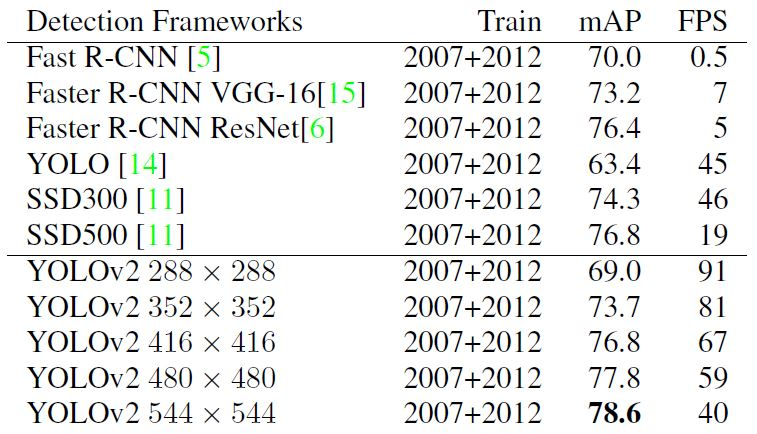
\includegraphics[width=0.5\textwidth]{comparativa_yolo}
\caption{Comparativa entre los distintos sistemas de detección de objetos sobre el mismo conjunto de entrenamiento y sobre la misma configuración \cite{yolov2}.}
\label{fig:3.2.13}
\end{figure}


% Por aclarar más cosas
\capitulo{4}{Técnicas y herramientas}

%Esta parte de la memoria tiene como objetivo presentar las técnicas metodológicas y las herramientas de desarrollo que se han utilizado para llevar a cabo el proyecto. Si se han estudiado diferentes alternativas de metodologías, herramientas, bibliotecas se puede hacer un resumen de los aspectos más destacados de cada alternativa, incluyendo comparativas entre las distintas opciones y una justificación de las elecciones realizadas. 
%No se pretende que este apartado se convierta en un capítulo de un libro dedicado a cada una de las alternativas, sino comentar los aspectos más destacados de cada opción, con un repaso somero a los fundamentos esenciales y referencias bibliográficas para que el lector pueda ampliar su conocimiento sobre el tema.

En esta sección se explican las distintas técnicas y herramientas utilizadas para llevar a cabo el proyecto.

\section{Lenguajes de programación}\label{tecyher}

\subsection{\textit{Python}}
\textit{Python}, versión 3.5, es el lenguaje de programación principal utilizado para el desarrollo de este proyecto. \textit{Python} es un lenguaje de alto nivel, interpretado, estructurado y de código abierto que puede ser usado para tareas de muchos tipos \cite{wiki:python}.

\textit{Python} se caracteriza por muchos aspectos. Y tiene múltiples ventajas respecto a otros lenguajes, como la fácil legibilidad de su código, las potentes funciones que incorpora por defecto, la utilización de tipado dinámico y las múltiples librerías de código abierto disponibles para distintas tareas, entre otras. Las ventajas que presenta respecto a otros lenguajes, como pueden ser C o Java, nos llevan a usar este lenguaje como el núcleo de nuestro proyecto.

\subsection{\textit{JavaScript}}
\textit{JavaScript} es el lenguaje de programación de \textit{HTML} y de la \textit{Web}~\cite{w3schools:javascript}. En nuestro caso, este es utilizado para la realización del etiquetador de imágenes, puesto que está basado en una aplicación \textit{Web}. No existen alternativas estándar a él. Pero sí existen librerías para facilitar el uso del mismo, como \textit{JQuery}, la cual es utilizada en la medida de lo posible.

\subsection{\textit{JSON}}
\textit{JSON}, siglas que denotan \textit{JavaScript Object Notation}, es un formato ligero para el intercambio de datos \cite{json}. Se basa en la notación de objetos de \textit{JavaScript}, de ahí su nombre. Este es utilizado para el almacenamiento de información en nuestra aplicación, como más tarde veremos.

Existe una posible alternativa a \textit{JSON}, la cual es \textit{XML}. Este es un lenguaje de marcado que puede ser utilizado con el mismo objetivo que \textit{JSON}. Pero \textit{XML} tiene distintas desventajas respecto \textit{JSON}:

\begin{itemize}
	\item \textit{JSON} es más corto.
	\item JSON es más facil de leer.
	\item JSON se integra facilmente con \textit{Python}\footnote{Python es capaz de traducir, o \textit{parsear}, \textit{JSON} a sus propias estructuras sin que tengamos que realizar ningun paso intermedio.}.
\end{itemize}
\section{\textit{Anaconda}}

\textit{Anaconda} es una distribución de \textit{Python} y \textit{R} que facilita las tareas de gestión de paquetes, de entornos y de versiones de lenguajes de programación. Nos permite crear varios entornos con distintas versiones de paquetes o lenguajes de programación. Y nos permite la instalación, desinstalación y actualización de distintos paquetes, facilitándonos estas tareas en la medida de lo posible.
 
\textit{Anaconda} nos proporciona muchas ventajas respecto a la utilización de \textit{Python} de manera aislada. La utilización de distintas versiones del mismo lenguaje en un mismo sistema operativo es una problemática que \textit{Anaconda} nos soluciona aislándonos de todos estos problemas. Además, como previamente se ha comentado sobre la gestión de paquetes, \textit{Anaconda} nos provee de una herramienta, \textit{<<conda>>}, para la gestión de paquetes.

En la realización de este proyecto se han utilizado múltiples paquetes, entre ellos: 

\begin{itemize}
	\item \textit{matplotlib}: usado para la representación de imágenes.
	\item \textit{numpy}: usado para facilitar la manipulación de vectores de números.
\end{itemize}
 
Adicionalmente, a continuación explico brevemente algunos otros paquetes con mayor influencia en el proyecto.
 
\subsubsection{\textit{scikit-image}}

\textit{scikit-image} nos proporciona un conjunto de herramientas para el procesamiento de imágenes. En las primeras fases, fue utilizada para distintos aspectos de investigación sobre la problemática a acometer, como la segmentación de imágenes. Pero finalmente, se utilizo para las tareas de \textit{data augmentation}, descriptores visuales, lectura y guardado de imágenes.

\subsection{\textit{scikit-learn}}
\textit{scikit-learn} nos proporciona un conjunto de herramientas para la minería de datos y análisis de estos. En concreto, esta se vio utilizada para la creación de clasificadores y para la realización de \textit{clustering}.

\subsubsection{\textit{Jupyter Notebook}}

Es una herramienta que nos permite crear \textit{webs} interactivas con código, texto, representaciones de los datos o distintas visualizaciones, como imágenes. Muchos de los productos generados por este proyecto serán de este tipo, como el etiquetador de imágenes.

\section{Librerías auxiliares}

Para llevar a cabo este proyecto, además de las librerías ya citadas, se han utilizado algunos repositorios auxiliares para llevar a cabo algunas de las tareas. Indico a continuación los repositorios con una breve descripción:

\begin{itemize}
	\item \textit{Jupyter Dashboards}: es una extensión que nos permitirá mostrar un \textit{Jupyter Notebook} con un estilo más personalizado.
	\item \textit{IPython File Upload}: es una extensión que nos permitirá subir imágenes desde un \textit{Jupyter Notebook}.
	\item \textit{darkflow}: es una implementación de \textit{YOLO} utilizado para el reconocimiento automático de fitolitos.
\end{itemize}

\subsection{Gestor de tareas: \textit{ZenHub}}

\textit{ZenHub} es una herramienta para la gestión de proyectos totalmente integrada con \textit{GitHub}. Esta herramienta nos permite obtener diagramas \textit{burndown}\footnote{Un diagrama \textit{burndown} es un gráfico que representa la cantidad de trabajo restante.} utilizados en el anexo de planificación del proyecto para el seguimiento del proyecto. También nos permite obtener un gráfico en el que podemos ver los puntos de historia\footnote{Los puntos de historia es una medida del esfuerzo a realizar para completar una tarea.} en los distintos \textit{sprints}\footnote{\textit{Sprint} es un periodo de tiempo en el que el conjunto de las tareas, definidas al principio de este, deben ser finalizadas y revisadas.}. Y, finalmente, nos proporciona un tablero \textit{kanban} para mejorar el flujo de trabajo.

\section{Control de versiones: \textit{Git}}

El control de versiones es una parte fundamental para la realización de un proyecto. Este nos permite acometer distintas acciones, como comprobar el cambio realizado entre versiones, trabajar en equipo fácilmente o volver a un punto anterior, entre otras cosas. En nuestro caso, utilizamos \textit{Git} como control de versiones. 

\textit{Git} nos proporciona las características que necesitamos. Además de algunas ventajas respecto a otras herramientas, como ser un sistema distribuido o proporcionar una interfaz de comandos muy potente.

%Y, además, tenía una experiencia básica con la herramienta. Lo cual, facilitaba la adopción de esta como herramienta de control de versiones.

\section{Repositorio: \textit{Github}}

Otra herramienta principal, a seleccionar, es el repositorio central, en nuestro caso hemos elegido \textit{Github}. \textit{Github} nos proporciona muchas utilidades y una forma simple de llevar a cabo el proyecto con todas las características necesarias. Es por todas sus características y una previa experiencia con la herramienta por lo que se eligió como nuestro servicio de repositorio central.

\section{Documentación: \LaTeX}

La memoria y anexos de este proyecto han sido escritos en \LaTeX. Este lenguaje de marcado nos proporciona muchas ventajas en contraste con otros editores de documentos, como \textit{Word} o sus alternativas, a la hora de realizar un documento de estas características.

\LaTeX\ nos facilita concentrarnos simplemente en el contenido. Supeditando a este la problemática de cómo debe formatearse el contenido. Por lo tanto, \LaTeX\ automatiza muchas de las típicas tareas que llevaríamos a cabo con otro editor de documentos y, además, permite obtener documentos con una altísima calidad.

\section{Entorno de desarrollo: \textit{JetBrains PyCharm}}

El entorno de desarrollo, o por sus siglas en inglés \textit{IDE}, es la aplicación utilizada para el desarrollo de la aplicación. Proporcionando múltiples herramientas, desde el auto-completar, hasta \textit{plugins} que permiten comprobar el recubrimiento del código mediante tests, entre otras funcionalidades.

Para esta utilidad se valoraron dos herrramientas principalmente: \textit{PyDev} y \textit{JetBrains PyCharm}. Escogiéndose esta última por poseer una mayor cantidad de herramientas integradas, como el control de versiones, distintas opciones para refactorizar el código y un muy buen auto-completar, entre otras características.

\section{Herramienta de prototipado: \textit{NinjaMock}}

La herramienta de prototipado es la aplicación utilizada para un primer diseño de la interfaz de una aplicación, facilitando la demostración, evaluación y agilizando el proceso de llevar a cabo una interfaz. En nuestro caso se utilizó \textit{NinjaMock}, la cual es una aplicación web que nos permite llevar a cabo esta tarea facilmente.
\capitulo{5}{Aspectos relevantes del desarrollo del proyecto}

En este apartado se recogen los detalles con mayor importancia en el desarrollo del proyecto. Tratando de mantener un orden cronológico con el que observemos los pasos que hemos seguido para solucionar las problemáticas del trabajo.

\begin{comment}
Este apartado pretende recoger los aspectos más interesantes del desarrollo del proyecto, comentados por los autores del mismo.
Debe incluir desde la exposición del ciclo de vida utilizado, hasta los detalles de mayor relevancia de las fases de análisis, diseño e implementación.
Se busca que no sea una mera operación de copiar y pegar diagramas y extractos del código fuente, sino que realmente se justifiquen los caminos de solución que se han tomado, especialmente aquellos que no sean triviales.
Puede ser el lugar más adecuado para documentar los aspectos más interesantes del diseño y de la implementación, con un mayor hincapié en aspectos tales como el tipo de arquitectura elegido, los índices de las tablas de la base de datos, normalización y desnormalización, distribución en ficheros3, reglas de negocio dentro de las bases de datos (EDVHV GH GDWRV DFWLYDV), aspectos de desarrollo relacionados con el WWW...
Este apartado, debe convertirse en el resumen de la experiencia práctica del proyecto, y por sí mismo justifica que la memoria se convierta en un documento útil, fuente de referencia para los autores, los tutores y futuros alumnos.
\end{comment}

\section{Procesamiento de imágenes}
\label{procimg}
Como primera aproximación al problema que nos concierne, nos hemos enfrentado al procesamiento de imágenes mediante la librería \textit{Scikit-image} de \textit{Python}. Mediante esta herramienta trataremos de dar solución a nuestro problema siguiendo los siguientes pasos:

\begin{enumerate}[1.]
  \item Convertir la imagen a escala de grises
  \item Segmentar los objetos del fondo de la imagen
  \item Obtener los distintos objetos de la imagen
\end{enumerate}

\subsection{Convertir la imagen a escala de grises}

La conversión de la imagen original (RGB) a escala de grises viene motivada con el mero objetivo de poder segmentar los objetos del fondo de la imagen mediante el método de \textit{Thresholding}. Solo pudiéndose partir de una imagen en escala de grises. En la figura \ref{fig:5.1.1} podemos ver los resultados.

\begin{figure}
	\centering
	\begin{subfigure}[b]{0.45\textwidth}
        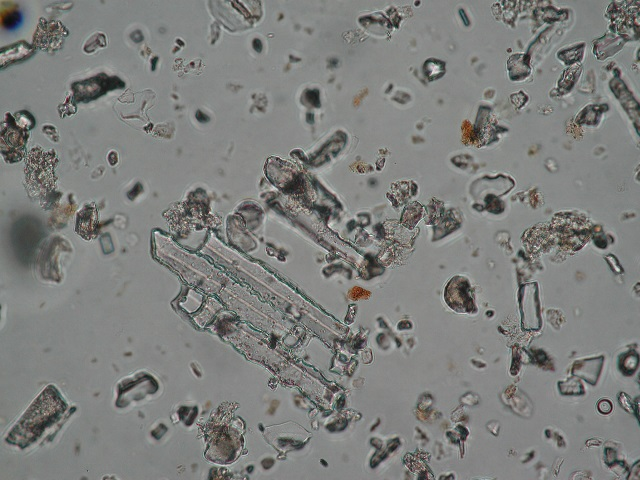
\includegraphics[width=\textwidth]{2}
        \caption{Original}
    \end{subfigure}
    \begin{subfigure}[b]{0.45\textwidth}
        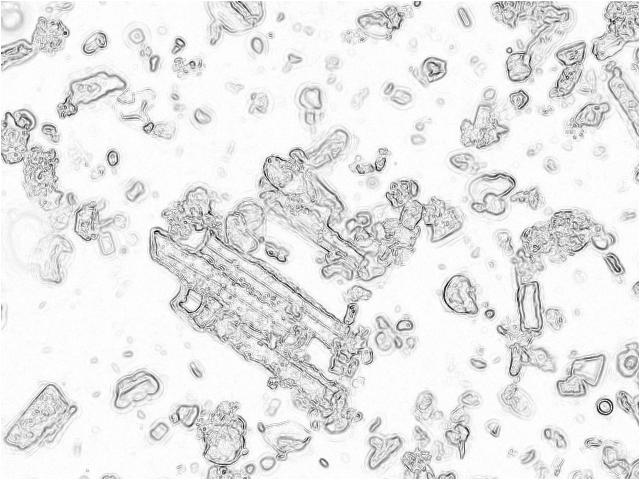
\includegraphics[width=\textwidth]{grayscale_image}
        \caption{Imagen en escala de grises}
    \end{subfigure}
    \caption{Conversión de la imagen original a escala de grises}
	\label{fig:5.1.1}
\end{figure}

\subsection{Segmentar los objetos del fondo de la imagen}

Una vez tenemos la imagen en escala de grises, procedemos a transformar nuestra imagen en una imagen en blanco y negro o binarizada. Los motivos por los que binarizamos la imagen es para obtener una imagen que sea más significativa para nosotros y además este simplificada. Lo cual nos será útil para facilitarnos su procesamiento.

\textit{Scikit-image} nos propociona distintos métodos mediante los cuales podemos segmentar una imagen. En la figura \ref{fig:5.1.2} podemos observar el resultado aplicando distintos métodos, los cuales se van indicando en cada una de las figuras.

\begin{figure}
	\centering
	\begin{subfigure}[b]{0.45\textwidth}
        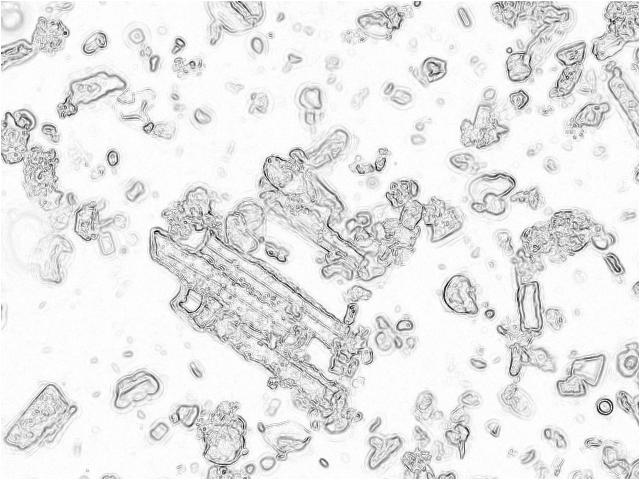
\includegraphics[width=\textwidth]{grayscale_image}
        \caption{Imagen en escala de grises}
    \end{subfigure}
    \begin{subfigure}[b]{0.45\textwidth}
        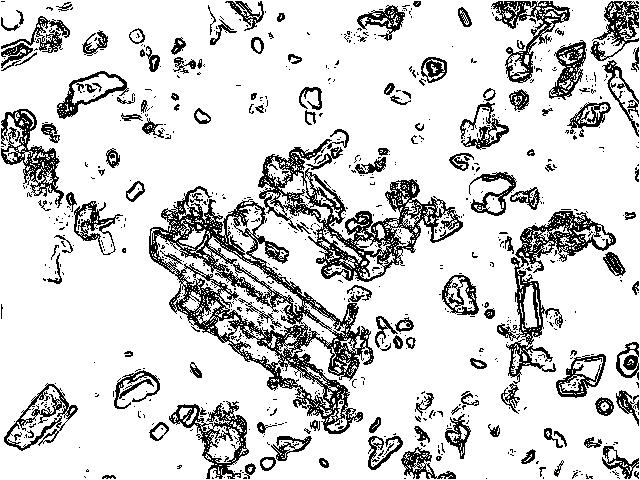
\includegraphics[width=\textwidth]{otsu_threshold_image}
        \caption{Método de Otsu}
    \end{subfigure}
    \begin{subfigure}[b]{0.45\textwidth}
        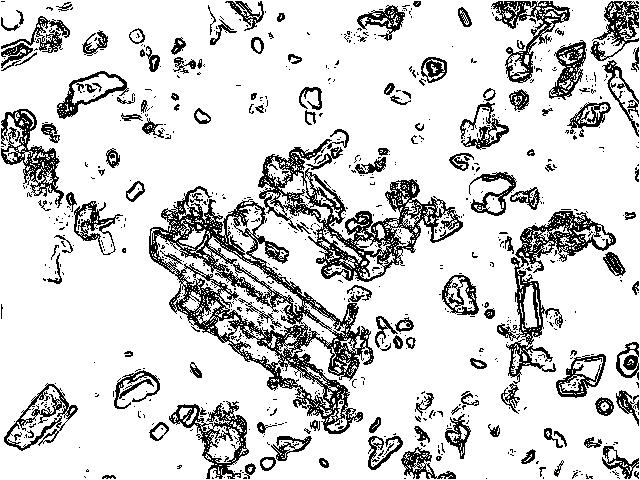
\includegraphics[width=\textwidth]{otsu_threshold_image}
        \caption{Método de Otsu}
    \end{subfigure}
    \begin{subfigure}[b]{0.45\textwidth}
        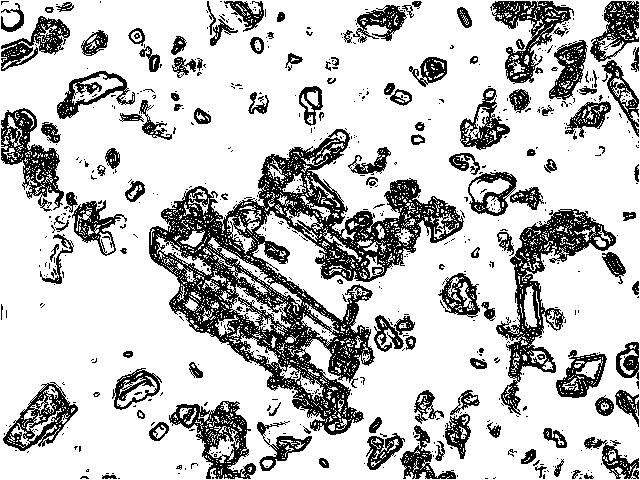
\includegraphics[width=\textwidth]{yen_image}
        \caption{Método de Yen}
    \end{subfigure}
    \begin{subfigure}[b]{0.45\textwidth}
        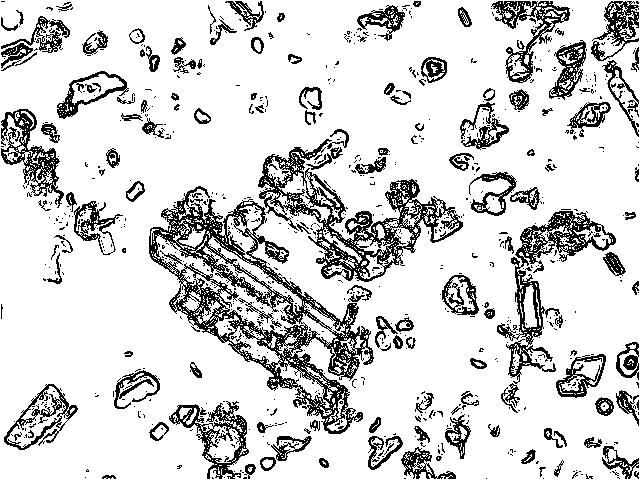
\includegraphics[width=\textwidth]{li_thresholded_image}
        \caption{Método de Li}
    \end{subfigure}
    \begin{subfigure}[b]{0.45\textwidth}
        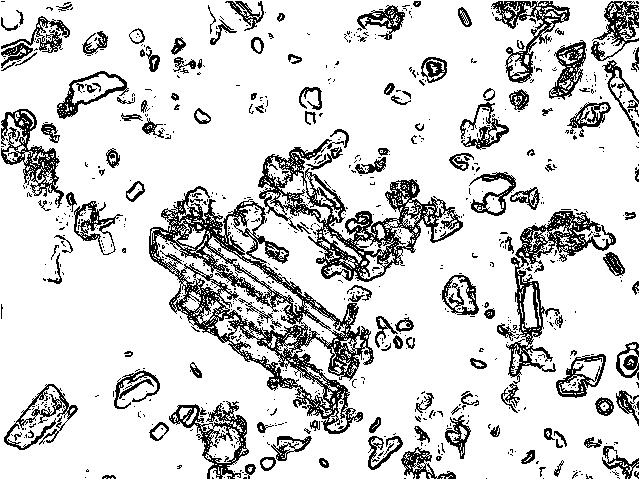
\includegraphics[width=\textwidth]{isodata_thresholded_image}
        \caption{Método de ISODATA}    
    \end{subfigure}
    \begin{subfigure}[b]{0.45\textwidth}
        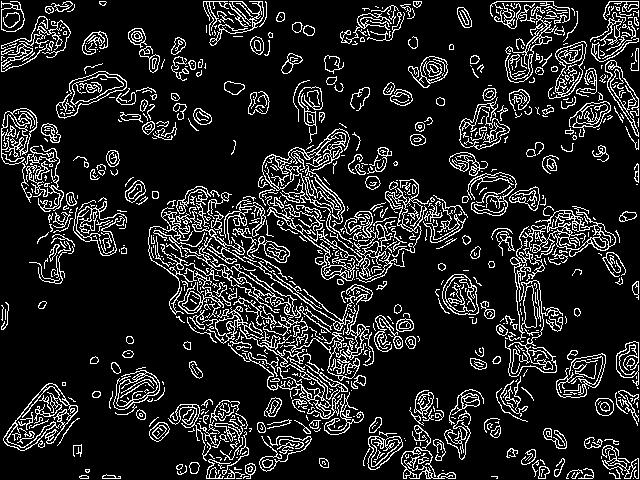
\includegraphics[width=\textwidth]{edge_based_image}
        \caption{Método basado en bordes}    
    \end{subfigure}
    \begin{subfigure}[b]{0.45\textwidth}
        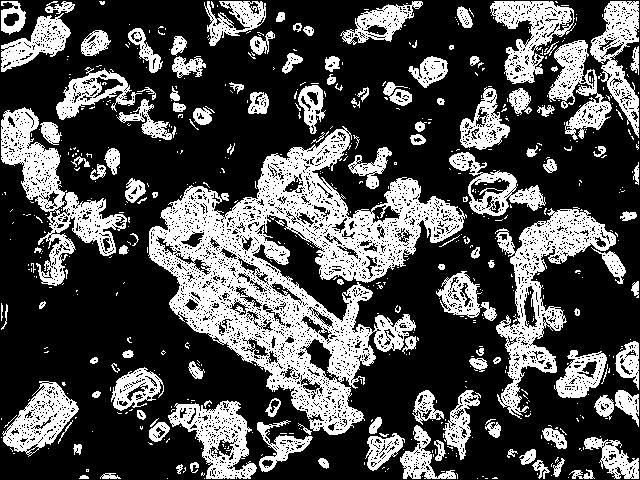
\includegraphics[width=\textwidth]{adaptive_thresholded_image_5}
        \caption{Método adaptativo}    
    \end{subfigure}
    \caption{Distintos ejemplos de una imagen segmentada}
	\label{fig:5.1.2}
\end{figure} 

\subsection{Obtener los distintos objetos de la imagen}
Después de tener la imagen binarizada de la forma más apropiada posible probamos a segmentar los distintos objetos de nuestra imagen.

\subsection{Transformación divisoria}
Transformación divisoria, o en inglés \textit{Watershed segmentation}, es un algoritmo clásico para la segmentación de objetos en una imagen~\cite{wiki:watershed}.

Durante las primeras pruebas, la segmentación más interesante hasta el momento ha sido la que se muestra en la figura \ref{fig:5.1.3}. A partir de \textit{Watershed segmentation} con marcado, representando cada color un objeto distinto. Más allá de esta segmentación no se ha conseguido nada mejor.

\begin{figure}
	\centering
	\begin{subfigure}[b]{0.45\textwidth}
        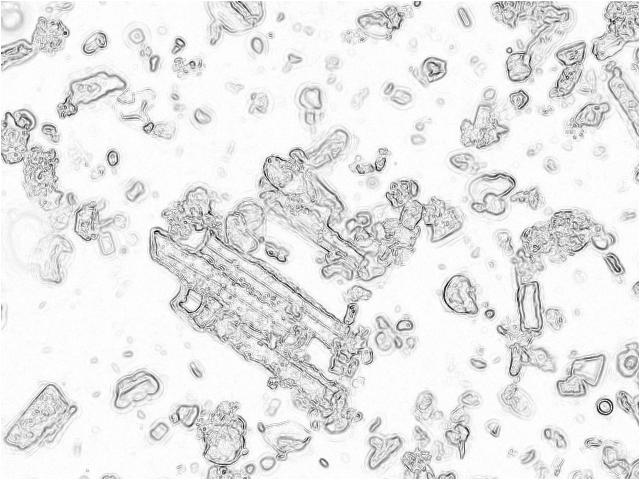
\includegraphics[width=\textwidth]{grayscale_image}
        \caption{Imagen en escala de grises}
    \end{subfigure}
    \begin{subfigure}[b]{0.45\textwidth}
        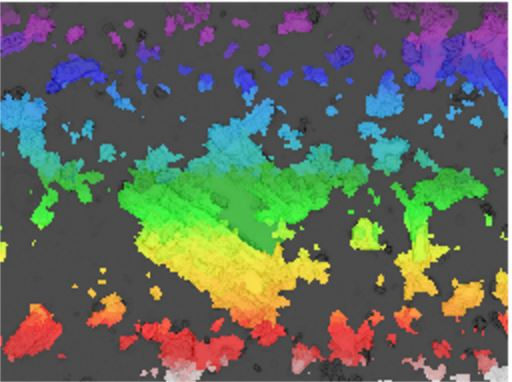
\includegraphics[width=\textwidth]{segmented}
        \caption{Imagen segmentada}
    \end{subfigure}
        \caption{Resultados obtenidos mediante transformación divisoria}
	\label{fig:5.1.3}
\end{figure} 	

\section{Problema fundamental: falta de imágenes}

Llegados a este punto, y teniendo una primera aproximación, con mayor o menor precisión, de como afrontar el reconocimiento automático de fitolitos, se plantea un problema fundamental en el desarrollo de este proyecto. El problema, al que me refiero, es que no poseemos o conocemos ningún conjunto de entrenamiento de imágenes etiquetadas\footnote{Me refiero por imágenes etiquetadas, a imágenes con las coordenadas de donden se encuentran los distintos fitolitos en estas.} de fitolitos. Y por lo que hemos podido observar, hasta el momento, es el requisito básico en el aprendizaje supervisado.

Debido a esta problemática, desarrollamos un etiquetador de fitolitos que permita a nuestros usuarios crear un conjunto de imágenes de fitolitos etiquetadas y así, solucionar este problema fundamental en el desarrollo del proyecto.

En concreto, este etiquetador es una aplicación web desarrollada sobre un conjunto de tecnologías \textit{Python} y \textit{JavaScript}. Con el objetivo de poder realizar un futuro despliegue en un servicio \textit{web} que facilite lo máximo las tareas a nuestros usuarios. Aunque en su desarrollo resulto en un problema, por la falta de manuales que enseñasen como llevarlo a cabo y la complejidad que introduce la comunicación entre \textit{Python} y \textit{JavaScript}. La información más detallada para un futuro programador, o para el uso por parte del usuario, se encuentra en los anexos del manual del programador y el manual del usuario, respectivamente.

\section{Clasificadores}

La aproximación mediante procesamiento de imágenes, mostrada previamente en la sección \ref{procimg}, no parece la más adecuada visto los resultados obtenidos. Por ello vamos a realizar el estudio sobre una segunda aproximación  mediante clasificadores, junto a descriptores visuales y la técnica de la ventana deslizante, o en inglés \textit{sliding window}.

\textit{Sliding window} consiste en la subdivisión de una imagen en distintos fragmentos, estableciendo previamente el tamaño de los fragmentos, tanto en ancho como en alto, y el tamaño del salto en cada eje, tras una subdivisión. 

Como podemos apreciar en la figura \ref{fig:sliding_window}, primero la ventana deslizante recorre la imagen en el eje horizontal. Comenzando por la esquina superior izquierda hasta llegar a la esquina superior derecha. Generando una imagen por cada subdivisión y realizando saltos horizontales según el tamaño que hayamos definido. Una vez esta llega a la esquina superior derecha, la ventana deslizante lleva a cabo el mismo proceso pero realizando un salto en el eje vertical. Y así sucesivamente hasta completar su recorrido por toda la imagen.

\begin{figure}
\centering
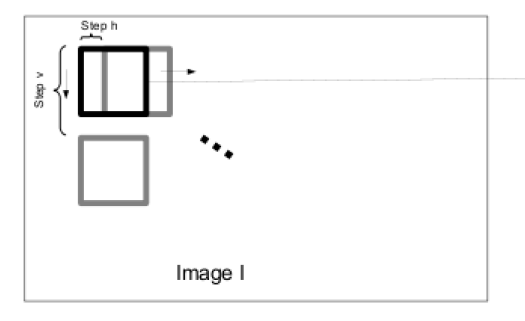
\includegraphics[width=0.8\textwidth]{sliding_window}
\caption{Esquema del funcionamiento de la ventana deslizante}
\label{fig:sliding_window}
\end{figure}

El primer conjunto de técnicas escogidas ha sido una Máquina de Vector Soporte(SVM)~\cite{svm} junto al Histograma de los gradientes orientados, la cual es una técnica para la extracción automática de características. Sin embargo, iremos utilizando distintas técnicas para adoptar la que mejor se adapte a nuestra problemática.

El procedimiento para obtener el clasificador es el siguiente:

\begin{enumerate}[1.]
  \item Crear un conjunto de entrenamiento de imágenes de caras que consideramos que son elementos positivos.
  \item Crear un conjunto de entrenamiento de imágenes de no-caras que consideramos que son negativos.
  \item Extraer las características del conjunto de entrenamiento  mediante un descriptor visual.
  \item Entrenar\footnote{Nos referimos por entrenar, en este ámbito, a enviar al clasificador las distintas imágenes con la clase a la que pertenecen (fitolito de tipo 1, fitolito de tipos 2, etc.).} el clasificador.
\end{enumerate}

 Finalizado el entrenamiento, ya tenemos nuestro clasificador listo para enviarle nuevas imágenes y que sean clasificadas.
 
\subsection{Reconocimiento de imágenes en nuevas imágenes}
Para el reconocimiento de objetos en nuevas imágenes, deberemos llevar a cabo los tres siguientes pasos:

\begin{enumerate}[1.]
  \item Dividir la imagen en múltiples fragmentos.
  \item Comprobar si cada uno de los fragmentos contiene el objeto.
  \item Si existe solapamiento en la detección de objetos, muy común en el uso de este tipo de clasificadores, se deben de combinar dichos solapamientos en uno único.
\end{enumerate}

Cada uno de los fragmentos anteriores se solapa en gran medida. Por lo que origina un problema de sobrereconocimiento de objetos, reconociendo donde existe un posible positivo, más de uno, en la mayoría de casos. Por ello, se aplica el tercer paso sobre los objetos reconocidos, que es la eliminación del solapamiento de objetos mediante la técnica de \textit{Non-maximum suppression}.

\subsection{Aplicación sobre el reconocimiento de caras}

Como previa experimentación con esta metodología, vamos a entrenar el clasificador para el reconocimiento de caras. Y en función de la efectividad del método sobre las caras tomaremos una serie de conclusiones sobre las que decidiremos si llevar a cabo esta solución sobre  nuestro problema.

Como explicábamos anteriormente, una vez tenemos nuestro clasificador le enviamos una nueva imagen, como podría ser la presentada en la figura \ref{subfig:family}. A partir de esta imagen el clasificador nos permitirá obtener las ventanas \footnote{Se entiende por ventana, en este contexto, a la caja o cuadrilátero que etiqueta un positivo en una imagen.} en las que detecta una cara, como vemos en la figura \ref{subfig:family_labeled}. Podemos apreciar que existe más de una ventana alrededor de cada cara. Y finalmente, tras aplicar el método \textit{Non-Maximum supresion} obtenemos el resultado final mostrado en la figura \ref{subfig:family_labeled_nms}.

\begin{figure}
	\centering
	\begin{subfigure}[b]{0.45\textwidth}
        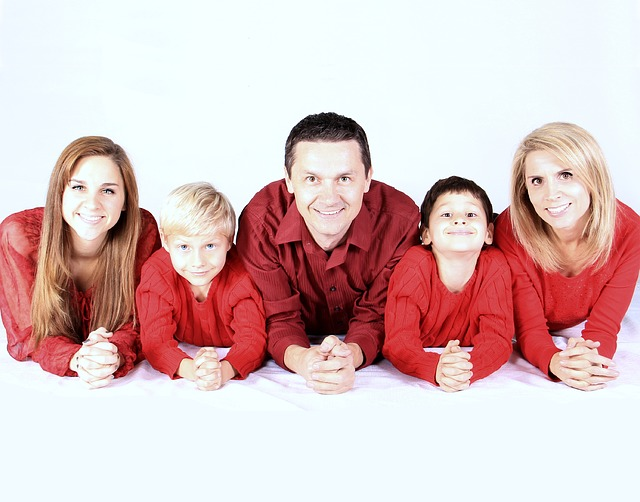
\includegraphics[width=\textwidth]{family}
        \caption{Imagen original}
        \label{subfig:family}
    \end{subfigure}
    \begin{subfigure}[b]{0.45\textwidth}
        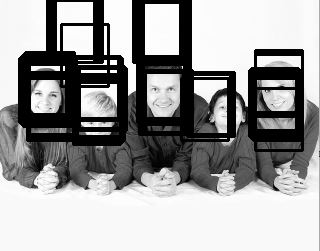
\includegraphics[width=\textwidth]{family_labeled}
        \caption{Imagen después de aplicarla nuestro clasificador}
        \label{subfig:family_labeled}
    \end{subfigure}
    \begin{subfigure}[b]{0.45\textwidth}
        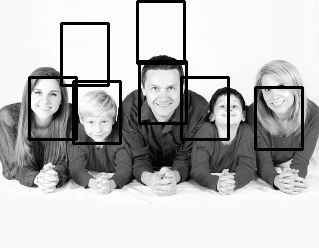
\includegraphics[width=\textwidth]{family_labeled_nms}
        \caption{Imagen tras aplicarla \textit{Non-Maximum supresion}}
         \label{subfig:family_labeled_nms}
    \end{subfigure}
        \caption{Resultados tras aplicar el clasificador sobre una imagen}
	\label{fig:5.1.4}
\end{figure}

\section{Conclusiones}

El método utilizado en esta sección se encuentra muy limitado por los siguientes aspectos:

\begin{itemize}
	\item Es una técnica que presenta problemas de rendimiento. Puesto que requiere de 2 o 3 segundos, como mínimo, para clasificar una nueva imagen.
	\item Es una técnica que no tiene en cuenta el contexto de la imagen para su clasificación. Sino, que solo tiene en cuenta cada uno de los fragmentos de la imagen de manera aislada al resto. Lo cual dificulta una adecuada precisión del clasificador.
	\item Comete muchos errores en la detección de falsos positivos. Como se puede observar en la figura \ref{subfig:family_labeled_nms}.
	\item El tamaño de la subdivisión de la imagen es constante. Por lo tanto, complica las posibilidades en la detección de distintos tamaños de fitolitos.
\end{itemize}

\section{Detección de objetos mediante técnicas de \textit{deep learning}}

Una vez observados los resultados mediante una técnica clásica, como es \textit{sliding window}. Vamos a ir un paso más allá, con las técnicas de \textit{deep learning}, las cuales son las que,  con diferencia, mayor rendimiento aportan en la actualidad, como previamente he explicado en los conceptos teóricos.

Para ello, vamos a entrenar una implementación de \textit{YOLO} en \textit{Python}, todavía en desarrollo, para tratar de llevar a cabo el detector automático de fitolitos. Aunque, existen otras alternativas que se podrían adoptar en un fúturo de no conseguir los resultados esperados con esta implementación.

Previamente, en los conceptos teóricos, se ha explicado que este tipo de modelos también presentan algunas problemáticas, por el volumen de imágenes necesario y el tiempo necesario para ser entrenados, principalmente. Existen soluciones, como \textit{data augmentation}, trasferencia de conocimiento o partir de modelos previamente entrenados. Que iremos valorando en este desarrollo.
\capitulo{6}{Trabajos relacionados}

%Este apartado sería parecido a un estado del arte de una tesis o tesina. En un trabajo final grado no parece obligada su presencia, aunque se puede dejar a juicio del tutor el incluir un pequeño resumen comentado de los trabajos y proyectos ya realizados en el campo del proyecto en curso. 

Actualmente, no existe ningún sistema popular que intente solucionar el problema acometido en este trabajo. Pero si existen trabajos similares en los que se estudian posibles técnicas para abordar la realización de sistemas automáticos para materiales microscópicos \cite{palyrecog}.

En el caso del artículo \textit{Automatic recognition of complete palynomorphs in digital images} \cite{palyrecog}, escrito por J.J. Charles, se crea un sistema consistente en las siguientes tres fases:

\begin{enumerate}
	\item Preprocesar la imagen, segmentando la parte de atrás de la imagen de la parte de delante.
	\item Segmentar las distintas regiones de la imagen.
	\item Clasifica las regiones de la imagen.
\end{enumerate}

Esta aproximación genera muy buenos resultados para la aplicación estudiada, pero presenta varios problemas para nuestro caso. Los problemas a los que me refiero son los siguientes:

\begin{itemize}
	\item Es un sistema aplicado a una única clase de objetos. En nuestro caso, queremos que sea un sistema escalable debido a la gran variedad de tipos de fitolito.
	\item No existen grandes diferencias en los tamaños de palinofaceos. Fue entrenado para objetos de tamaño 30, 50 y 70. Pero en nuestro caso los fitolitos son de distintos tamaños, estrechos y altos, o viceversa. Es decir, teniendo tamaños muy variados y siendo tridimensionales, por lo cual las formas de los materiales varían sustancialmente. Lo cual complica nuestro proyecto un gran paso más allá.
	\item En ningun momento se hace referencia al tiempo necesario para clasificar una nueva imagen. Pero estas técnicas sueles ser bastante ineficientes, debido al gran espacio de exploración que plantean.
\end{itemize}

Por lo tanto, las técnicas de \textit{deep learning} actuales presentan grandes mejoras en cuanto a eficiencia, escalabilidad, y flexibilidad en cuanto al aprendizaje de nuevos tipos de fitolitos, en nuestro caso. Aunque también presentan otros problemas a cambio de sus grandes posibilidades, como he comentado previamente en otras secciones.
\capitulo{7}{Conclusiones y Líneas de trabajo futuras}

%Todo proyecto debe incluir las conclusiones que se derivan de su desarrollo. Éstas pueden ser de diferente índole, dependiendo de la tipología del proyecto, pero normalmente van a estar presentes un conjunto de conclusiones relacionadas con los resultados del proyecto y un conjunto de conclusiones técnicas. 
%Además, resulta muy útil realizar un informe crítico indicando cómo se puede mejorar el proyecto, o cómo se puede continuar trabajando en la línea del proyecto realizado. 

\section{Conclusiones}

\section{Lineas futuras de trabajo}

Los fitolitos poseen una complejidad enorme por la multitud de formas de estos, incluso perteneciendo a un mismo tipo, y la multitud de tipos de fitolitos existentes. Por lo tanto, existe un gran margen de mejora en el reconocimiento automático de estos.

El problema fundamental, junto al ya expuesto sobre la complejidad de las formas de los fitolitos, es la inexistencia de un conjunto de imágenes etiquetadas de fitolitos. Actualmente, las técnicas más avanzadas para el reconocimiento de objetos necesitan de conjuntos de entrenamiento muy grandes. Por ello, en futuros desarrollos se podrían mejorar las técnicas de \textit{data augmentation} e incorporar nuevas técnicas con el objetivo de obtener un conjunto de entrenamiento sustancialmente mayor.

Una de las nuevas técnicas a las que me refiero es el aprendizaje mediante modelos 3D, el cual nos permitiría crear un conjunto de imágenes significativamente mayor~\cite{sem}~\cite{3dmodels}. Estas técnicas consiguen recrear un modelo 3D de un objeto a partir de diferentes imágenes. Y a partir del modelo generado obtener imágenes desde las distintas perspectivas.

Otra posible mejora sería la realización del entrenamiento de \textit{YOLO} en un entorno con mayores recursos, sobre todo con la utilización de una mejor tarjeta gráfica, como la \textit{Nvidia Titan X}. O incluso con la utilización de varias tarjetas gráficas concurréntemente, lo cual aceleraría el proceso de entrenamiento significativamente.


\bibliographystyle{plain}
\bibliography{bibliografia}

\end{document}
